\documentclass{beamer}

%For 16:10 screens/projectors
%\usepackage[orientation=landscape,size=custom,width=16,height=10,scale=0.5,debug]{beamerposter} 

\mode<presentation>
{
  \usetheme{Madrid}
  \setbeamercovered{transparent}
}
%\useoutertheme{infolines}


\usepackage[english]{babel}
\usepackage[latin1]{inputenc}
\usepackage{amsmath}
\usepackage{multimedia}
\usepackage{pgf}
\usepackage{pst-gantt}
\usepackage{graphicx,color,psfrag}
\DeclareGraphicsExtensions{.png,.jpg}
\usepackage{pstricks}
\usepackage{epsf,multirow,textcomp}
\usepackage{algorithm,algorithmic}
\usepackage{epstopdf}


\title[Feature Learning with Neural Nets]{\Large{Improved Music Feature Learning with Deep Neural Networks} }

\author[S. Sigtia and S. Dixon]{Siddharth Sigtia and Simon Dixon\\ \texttt{\scriptsize{\{sss31,simond\}@qmul.ac.uk}}}

\institute[C4DM]{Centre for Digital Music\\Queen Mary University of London}

\date{}

%Left logo
\pgfdeclareimage[height=0.4cm]{c4dm}{Figures/c4dm.eps}
\setbeamertemplate{sidebar left}{
   \vfill
   \rlap{\hskip0.1cm \href{http://www.elec.qmul.ac.uk/digitalmusic/index.html}{\pgfuseimage{c4dm}}}
   \vskip2pt
   \llap{\usebeamertemplate***{navigation symbols}\hskip0.1cm}
   \vskip2pt
} 

%Right logo
\logo{
\includegraphics[height=0.5cm]{Figures/qm_blue_logo.eps}}


\begin{document}

\begin{frame}
  \titlepage


  
\end{frame}


\section{Introduction}


\begin{frame}{Motivation}
\vspace{-0.15in}
  \begin{itemize}
  \item Try to learn the most optimal features for a particular task and reduce dependency on hand-crafted features.
  \item {\usebeamercolor[fg]{structure} How can we learn features for a particular task?}:
    \\Neural nets with several hidden layers (deep networks) provide a way to learn features for a particular task.  
  \item {\usebeamercolor[fg]{structure} Can we learn features for MIR tasks with neural nets?}: 
    \\Lots of recent evidence suggests yes! 
    \\Neural nets have been used to successfully learn features for genre classification (Hamel,Sander), Music Transcription, Emotion prediction, music prediction etc. 

  \end{itemize}
\end{frame}

\begin{frame}{Challenges}
Optimisation
%{\usebeamercolor[fg]{structure}Optimisation}
  \begin{itemize}
    \item Training neural networks with several hidden layers is challenging. 
    \item The optimisation problem is highly non-linear and the best we can do is hope to find a useful local minimum. 
    \item Unsupervised pre-training helps optimisation by finding a good initial parameter set.
    \item The number of hyper-parameters can be quite large if we include momentum, learning rate schedules etc.   
  \end{itemize}
\end{frame}

\begin{frame}{Current State of the Art}
  \begin{itemize}
    \item The use of neural networks for supervised learning has come full circle in some ways.
    \item Unsupervised pre-training is not considered to be necessary for finding good solutions. 
    \item Gradient based optimisers starting with random parameter initialisation provide good results. 
    \item Rectified linear units, Dropout, Hessian Free optimisation, Nesterov's accelerated gradient have all been applied successfully to various problems. 
  \end{itemize}
\end{frame}

\begin{frame}{Problem Definition}
We evaluate our ideas on a genre classification problem. 
Insert a figure of the genre-classification pipeline. 
3 boxes, feature extraction, classification, pooling, something like that. 
Maybe colour the feature extraction box. 
\end{frame}

\begin{frame}{Rectified Linear Units}
Maybe just pictures? One of the activation function, one of the gradients passing. maybe mention why the gradients flow better. 
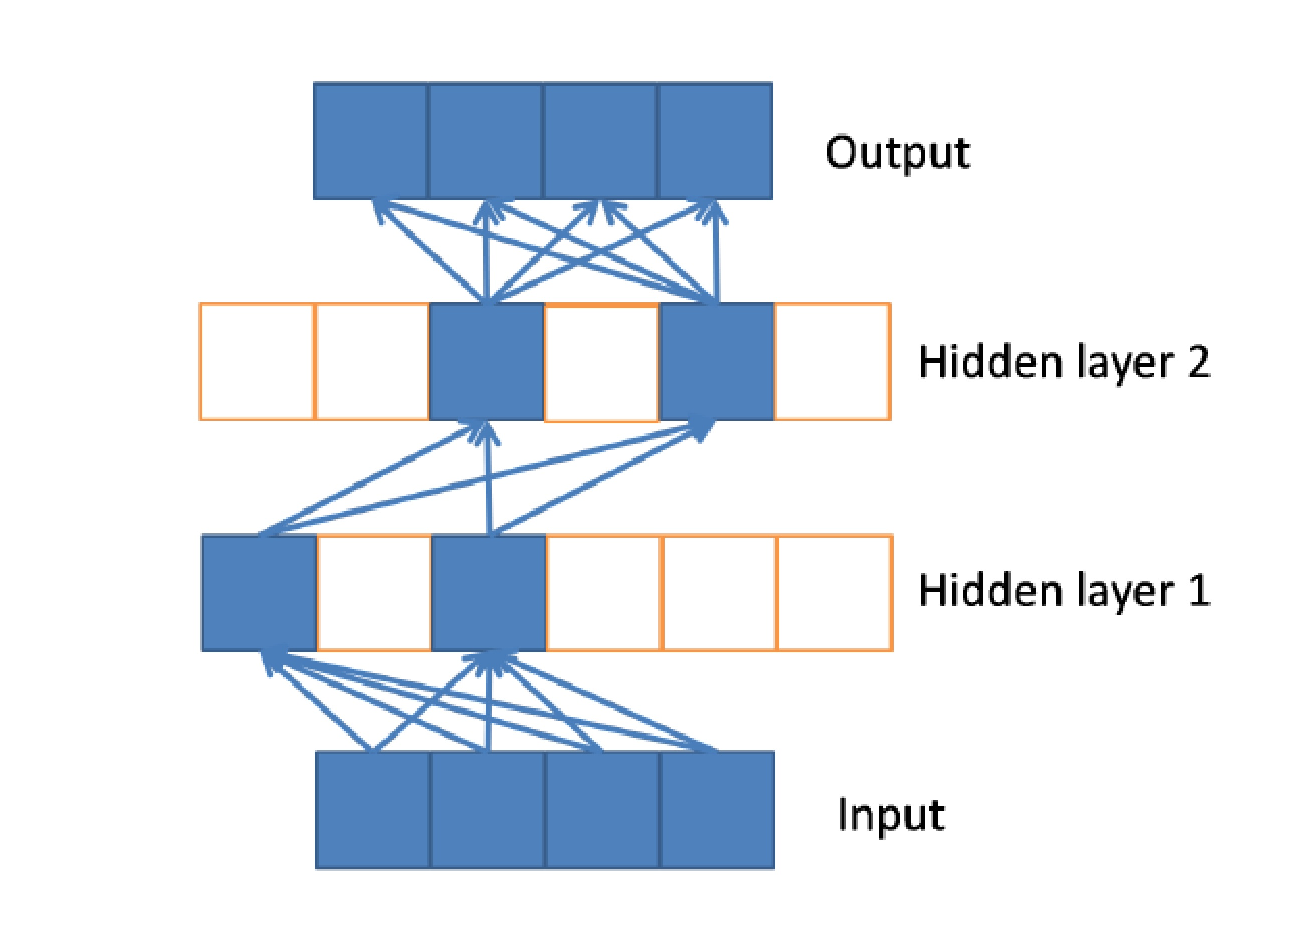
\includegraphics[scale=0.3]{Figures/ReLU-grads.eps}
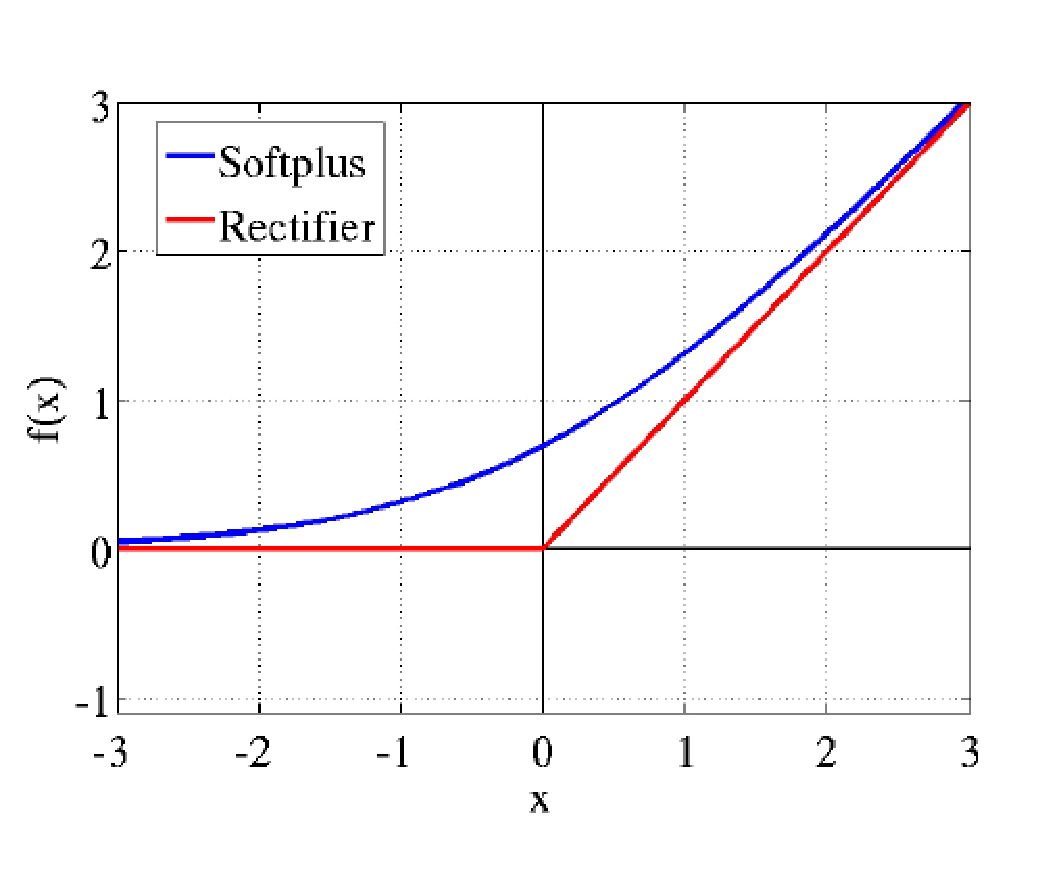
\includegraphics[scale=0.3]{Figures/ReLU-acts.eps}
\end{frame}

\begin{frame}{Dropout}
\end{frame}

\end{document}



